% Author: Izaak Neutelings (June, 2018)
\documentclass[border=3pt,tikz]{standalone}
\usepackage{ifthen}
\usepackage{siunitx}
\usepackage{tikz}
\usetikzlibrary{hobby} % for ..
\usetikzlibrary{arrows.meta} % to control arrow size
\usetikzlibrary{decorations.text}
\tikzset{>={Latex[length=4,width=4]}} % for LaTeX arrow head
\usetikzlibrary{calc,intersections,decorations.markings}
\usepackage{siunitx}
\usepackage{xcolor} % for colored text

\colorlet{mylightblue}{blue!20}
\colorlet{myblue}{blue!50!black}
\colorlet{mydarkblue}{blue!30!black}
\colorlet{mylightred}{red!10}
\colorlet{myred}{red!50!black}
\colorlet{mydarkred}{red!60!black}
\colorlet{mydarkgreen}{green!30!black}

%\tikzstyle{midarr}=[decoration={markings,mark=at position 0.5 with {\arrow{stealth}}},postaction={decorate}]
\tikzset{
    midarr/.style={decoration={markings,mark=at position #1 with {\arrow{stealth}}},postaction={decorate}},
    midarr/.default=0.5
}
\def\tick#1#2{\draw[thick] (#1) ++ (#2:0.03*\ymax) --++ (#2-180:0.06*\ymax)}


\begin{document}

% PV diagram - Maxwell construction
    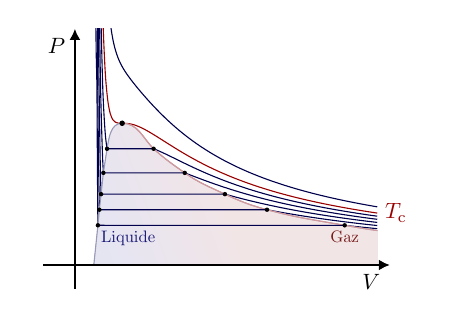
\begin{tikzpicture}
        \message{PV diagram - Maxwell construction^^J}
        \def\xmax{4}
        \def\ymax{3}
        \def\N{110}
        \def\s{0.6}
        \def\A{1.8}
        \def\isotherm#1#2{{ \A*(8*#2)/(3*#1-1) - 3*\A/(#1*#1) }} % reduced equation of state
        \coordinate (C) at (\s,\A);

        % LINE
        \foreach \i/\T/\pe in {0/.75/.28,1/.8/.39,2/.85/.5,3/.9/.65,4/.95/.82,5/1.0/1,6/1.1/1}{

            \begin{scope}
                \clip (-0.15*\xmax,0) rectangle (1.10*\xmax,\ymax);
                \ifthenelse{\i = 5}{
                    \draw[mydarkred,variable=\x,domain=0.36:{.96*\xmax/\s},range=0:1,samples=\N,smooth,name path=isotherm]
                    plot (\s*\x,\isotherm{\x}{\T}) node[mydarkred,right,scale=0.8] {$T_\text{c}$};
                }{
                    \draw[mydarkblue,variable=\x,domain=0.36:{.96*\xmax/\s},range=0:1,samples=\N,smooth,name path=isotherm]
                    plot (\s*\x,\isotherm{\x}{\T});
                }

                \ifthenelse{\i < 5}{ %\lengthtest{\pe pt < 1 pt}
                    \path[name path={pe}] (0,\A*\pe) --++ ({.96*\xmax/\s},0);
                    \path[name intersections={of=isotherm and pe,name=pe\i}];
                }

            \end{scope}
        }

        \begin{scope}
            \clip (0,0) rectangle (.96*\xmax,.96*\ymax);
            \fill[top color=myblue!10,bottom color=myred!10,middle color=myred!10,shading angle=110,
                draw=mydarkblue!40,thin,use Hobby shortcut]
            (.06*\xmax,0) -- (pe0-1) -- (pe1-1) -- (pe2-1) -- (pe3-1) --
            (pe4-1) to[out=80,in=180]
            (C) to[out=0,in=135]
            (pe4-3) to[out=-42,in=145]
            (pe3-3) to[out=-35,in=155]
            (pe2-3) to[out=-25,in=165]
            (pe1-3) to[out=-15,in=170]
            (pe0-3) to[out=-10,in=172]
            (.97*\xmax,.144*\ymax) |- (0,0);
            \draw[mydarkred!40,thin,use Hobby shortcut]
            (C) to[out=0,in=135]
            (pe4-3) to[out=-42,in=145]
            (pe3-3) to[out=-35,in=155]
            (pe2-3) to[out=-25,in=165]
            (pe1-3) to[out=-15,in=170]
            (pe0-3) to[out=-10,in=172]
            (.97*\xmax,.144*\ymax) |- (0,0);
        \end{scope}
        \node[blue!40!black!90,below right=-1,scale=0.6] at (pe0-1) {\strut Liquide};
        \node[red!40!black!90,below=-1,scale=0.6] at (pe0-3) {\strut Gaz};

        % MAXWELL CONSTRUCTION
        \fill (C) circle (1pt);
        \foreach \i in {0,1,2,3,4}{
            \draw[thin,mydarkblue] (pe\i-1) -- (pe\i-3);
            \fill[black] (pe\i-3) circle (.8pt);
            \fill[black] (pe\i-1) circle (.8pt);
        }

        % AXIS
        \draw[->,thick] (0,-0.1*\ymax) -- (0,\ymax)
        node[anchor=north east,inner sep=4,scale=0.8] {$P$};
        \draw[->,thick] (-0.1*\xmax,0) -- (\xmax,0)
        node[anchor=north east,inner sep=4,scale=0.8] {$V$};

    \end{tikzpicture}

\end{document}
